\documentclass[11pt]{amsart}

\usepackage[all]{xy}
\usepackage{amsmath,amssymb,amsthm}
\usepackage{tikz}

\usetikzlibrary{decorations.pathreplacing,decorations.markings}


\usepackage{xcolor}
\def\todoit{{\color{red} $^{TODO}$}} %!!!!!!!!!!!!!!!!!!!! I CHANGED YOUR COMMAND. !!!!!!!!!!!!!!!!!!!!
%%%%%%%%%%%%%%%%%%%%%%%%%%%%%%%%%%%%%%%%%%%%%%%%%%%%%%%%%%%%%%%%%%%%%%%%%%%%%%%%%%%%%%%%%%%%%%%%%%%%%%%
%I'm trying an alternate todo note setup that will give us a quick glance at start of document of those things that need doing. The relevant package is on the next line, and the List of Todos setup is right before the \begin{document} command.
%%%%%%%%%%%%%%%%%%%%%%%%%%%%%%%%%%%%%%%%%%%%%%%%%%%%%%%%%%%%%%%%%%%%%%%%%%%%%%%%%%%%%%%%%%%%%%%%%%%%%%%
\def\ltblue{blue!20!white}
\def\ltgreen{green!20!white}

\usepackage[colorinlistoftodos, textsize=tiny]{todonotes}

%\headheight 35pt
%
%\setlength{\textwidth}{6.5in}      %%%%%%%%%%%%%%%%%%%%%%%%%%%%%%%%%%%%%%%%%%%%%%%%%%%%%%%%%%%%%%%%%%%
%\setlength{\oddsidemargin}{0in}    Is it OK if we undo these formatting commands?
%\setlength{\evensidemargin}{0in}   %%%%%%%%%%%%%%%%%%%%%%%%%%%%%%%%%%%%%%%%%%%%%%%%%%%%%%%%%%%%%%%%%%%
%\setlength{\textheight}{8.5in}
%\setlength{\topmargin}{0in}
%\setlength{\headheight}{0in}
%\setlength{\headsep}{12pt}
%\setlength{\footskip}{.5in}

\renewcommand{\theenumi}{\roman{enumi}}

\tikzset{
  % style to apply some styles to each segment of a path
  on each segment/.style={
    decorate,
    decoration={
      show path construction,
      moveto code={},
      lineto code={
        \path [#1]
        (\tikzinputsegmentfirst) -- (\tikzinputsegmentlast);
      },
      curveto code={
        \path [#1] (\tikzinputsegmentfirst)
        .. controls
        (\tikzinputsegmentsupporta) and (\tikzinputsegmentsupportb)
        ..
        (\tikzinputsegmentlast);
      },
      closepath code={
        \path [#1]
        (\tikzinputsegmentfirst) -- (\tikzinputsegmentlast);
      },
    },
  },
  % style to add an arrow in the middle of a path
  mid arrow/.style={postaction={decorate,decoration={
        markings,
        mark=at position .5 with {\arrow[#1]{stealth}}
      }}},
}


\newcommand{\oarc}[4]{
\draw[thick, postaction={on each segment={mid arrow}}] (#1,#2) ..controls (#1 + .2,#2 + .7) and (#3 - .2,#4 + .7) .. (#3,#4);
}



\def\l{{\left(}}
\def\r{{\right)}}

\def\Z{{\mathbb Z}}
\def\C{{\mathbb C}}
\def\R{{\mathbb R}}
\def\D{{\mathbb D}}
\def\H{{\mathbb H}}
\def\P{{\mathbb P}}

\def\F{{\mathcal F}}
\def\M{{\mathcal M}}
\def\O{{\mathcal O}}
\def\A{{\mathcal A}}
\def\cl{\mathcal}

\def\s{{\sigma}}
\def\t{{\tau}}
\def\k{{\kappa}}

\def\g{\gamma}
\def\a{\alpha}
\def\xibar{\bar{\xi}}

\def\Xtilde{\widetilde{X}}
\def\etilde{\tilde{e}}

\def\bs{\backslash}
\def\dot{\bullet}

\def\G{{\Gamma}}
\def\SL{\mathrm{SL}}
\def\GL{\mathrm{GL}}
\def\O{\mathrm{O}}
\def\SO{\mathrm{SO}}
\def\U{\mathrm{U}}
\def\SU{\mathrm{SU}}
\def\PSL{\mathrm{PSL}}

\def\Gtilde{\widetilde{G}}
\def\SLtilde{\widetilde{\SL}}

\def\ar{\operatorname{ar}}
\def\mr{\operatorname{mr}}


\def\sing{{\mathrm{sing}}}

\newcommand\id{\operatorname{id}}
\newcommand\inter{\operatorname{int}}
\newcommand\Aut{\operatorname{Aut}}
\newcommand\Gal{\operatorname{Gal}}
\newcommand\rel{\operatorname{rel}}
\newcommand\Tr{\operatorname{Tr}}
\newcommand\End{\operatorname{End}}
\newcommand\diag{\operatorname{diag}}
\newcommand\Sp{\Sigma^{(p)}}

\newtheorem{thm}{Theorem}[section]
\newtheorem{lem}[thm]{Lemma}
\newtheorem{prop}[thm]{Proposition}
\newtheorem{cor}[thm]{Corollary}

\newenvironment{definition}[1][Definition]{\begin{trivlist}
\item[\hskip \labelsep {\bfseries #1}]}{\end{trivlist}}
\newenvironment{ex}[1][Example]{\begin{trivlist}
\item[\hskip \labelsep {\bfseries #1}]}{\end{trivlist}}
\newenvironment{rem}[1][Remark]{\begin{trivlist}
\item[\hskip \labelsep {\bfseries #1}]}{\end{trivlist}}

\makeatletter
\providecommand\@dotsep{5}
\def\listtodoname{List of Todos}
\def\listoftodos{\@starttoc{tdo}\listtodoname}
\makeatother

\begin{document}

\listoftodos
%%%%%%%%%%%%%%%%%%%%%%%%%%%%%%%%%%%%%%%%%%%%%%%%%%%%%%%%%%%%%%%%%%%%%%%%%%%%%%%%%%%%%%%%%%%%%%%%%%%%%%%%%
% BLUE is for David
% GREEN is for Cornwell
%%%%%%%%%%%%%%%%%%%%%%%%%%%%%%%%%%%%%%%%%%%%%%%%%%%%%%%%%%%%%%%%%%%%%%%%%%%%%%%%%%%%%%%%%%%%%%%%%%%%%%%%%
\newpage




%\title{The Augmentation Rank of Knot Cables}
%\author{David Hemminger\footnote{The author would like to thank Dr.\ Christopher Cornwell for the advising, and everyone else for the patience.}\\ Duke University}
%\maketitle

\begin{abstract}

\end{abstract}


\section{Introduction}
\todo[color=\ltblue,inline]{introduce corollary for iterated cables}
Let $K$ be a knot in $S^3$.  The \emph{meridional rank} of $K$, written $\mr(K)$, is the minimal size of a meridional generating set of the knot group of $K$.  It is bounded above by the bridge number $b(K)$, and Problem 1.11 of \cite{Kir95} asks whether $\mr(K) = b(K)$ for all knots $K$.  Cornwell has proven that the \emph{augmentation rank} $\ar(K)$ of $K$ (which is defined in Section \ref{SecBG}) bounds the meridional rank from below, and that $\ar(K) = \mr(K) = b(K)$ for some families of knots, including torus knots \cite{Cor13a}\todo[color=\ltgreen,inline]{labels and citations don't match}.


%Define ar
%generated by entries of $A_{ij}$

The main result of this paper is that if $\ar(K) = b(K)$ and $K$ is the closure of a braid with even writhe and index equal to $b(K)$, then the augmentation rank and bridge number are equal for any $(p,q)$-cable of $K$ where $\gcd(p,q) = 1$ and $p<q$.





\section{Background}
\label{SecBG}

We begin in Section \ref{SecBG_KCHdef} by reviewing the construction of $HC_0(K)$ from the viewpoint of the combinatorial knot DGA, which was first defined in \cite{Ng08}; our conventions are those given in \cite{Ng12}. In Section \ref{SecBG_AugRk} we discuss augmentations in knot contact homology and their rank, which gives a bound on the meridional rank of the knot group useful for studying the relation between meridional rank and bridge number. Finally, in Section \ref{SecBG_AugExist} is a discussion of techniques from \cite{Cor13b} that we use to calculate the augmentation rank.

\subsection{Knot contact homology}
\label{SecBG_KCHdef}

Let $\A_n$ be the noncommutative unital algebra over $\Z$ generated by $a_{ij}$, $1\le i\ne j\le n$.  Let $B_n$ be the braid group on $n$ strands, and define $\phi : B_n \rightarrow\Aut \A_n$ by defining it on the generators of $\A_n$ and extending by linearity

$$
\phi_{\s_k}\colon
\left\{
     \begin{array}{lr}
       a_{ij}\mapsto a_{ij} & i,j\ne k,k+1\\
       a_{k+1,i}\mapsto a_{ki} & i\ne k,k+1\\
       a_{i,k+1}\mapsto a_{ik} & i\ne k,k+1\\
       a_{k,k+1}\mapsto -a_{k+1,k} & \\
       a_{k+1,k}\mapsto -a_{k,k+1} & \\
       a_{ki}\mapsto a_{k+1,i} - a_{k+1,k}a_{ki} & i\ne k,k+1\\
       a_{ik}\mapsto a_{i,k+1} - a_{ik}a_{k,k+1} & i\ne k,k+1\\
     \end{array}
\right.
$$

Let $\iota\colon B_n \rightarrow B_{n+1}$ be the inclusion that adds in an $(n+1)$th strand that doesn't interact with the others, and define $\phi_B^*\in \Aut \A_{n+1}$ by $\phi_B^* = \phi_B\circ\iota$.  We then define the $n\times n$ matrices $\Phi_B^L$ and $\Phi_B^R$ with entries in $\A_n$ by

$$\phi_B^*(a_{i,n+1}) = \sum_{j=1}^n(\Phi_B^L)_{ij}a_{j,n+1}$$

$$\phi_B^*(a_{n+1,i}) = \sum_{j=1}^na_{n+1,j}(\Phi_B^R)_{ji}$$

We will need a relationship that exists between $\Phi_B^L$ and $\Phi_B^R$ in order to show that an augmentation is well-defined. To this end, define an operation $x\mapsto\overline x$ on $\A_n$ as follows: first $\overline{a_{ij}}=a_{ji}$; then, for any $x,y\in\A_n$, $\overline{xy}=\overline y\hspace*{1pt}\overline x$ and extend the operation linearly to $\A_n$.
\begin{prop}[\cite{Ng05}, Prop.\hspace*{-0.7pt} 6.2]For a matrix of elements in $\A_n$, let $\overline{M}$ be the matrix such that $\left(\overline M\right)_{ij} = \overline{M_{ij}}$. Then for $B\in B_n$, $\Phi_B^R$ is the transpose of $\overline{\Phi_B^L}$.
\label{Prop:Transpose}
\end{prop}

Let $\omega$ be the writhe of $B$, and define matrices $\bf{A}$ and $\Lambda$ by

\begin{equation}
\bf{A}_{ij} = 
\left\{
     \begin{array}{lr}
      a_{ij} & i<j\\
      -\mu a_{ij} & i>j\\
      1-\mu & i = j\\
     \end{array}
\right.
\label{def:Amatrix}
\end{equation}
\begin{equation}
\Lambda = \diag[\lambda\mu^\omega,1,\ldots,1].
\label{defn:Lambda}
\end{equation}

\begin{definition}
Suppose that $K$ is the closure of $B\in B_n$ and let $R_0$ be the Laurent polynomial ring $\Z[\lambda^{\pm 1},\mu^{\pm 1}]$. Define $\mathcal{I}\subset \A_n\otimes R_0$ to be the ideal generated by the entries of $\bf{A} - \Lambda\cdot\Phi_B^L\cdot \bf{A}$ and $\bf{A} - \bf{A}\cdot\Phi_B^R\cdot\Lambda^{-1}$.  The \emph{degree zero homology of the combinatorial knot DGA} is $\operatorname{HC}_0(K) = (\A_n\otimes R_0)/\mathcal{I}$.
\label{defn:HC_0}
\end{definition}
It was shown in \cite{Ng08} that the isomorphism class of $HC_0(K)$ is unchanged under the Markov moves, and hence provides an invariant of the knot $K$. While we only consider $HC_0(K)$ here, it is part of the larger invariant, the combinatorial knot DGA of $K$, studied in \cite{Ng08} which is a computation of the Legendrian contact homology of a Legendrian lift of $K$ to the cosphere bundle over $\R^3$ (\cite{EENS12}).

The following result, originally proved in \cite{Ng05}, on the behavior of the matrices $\Phi_B^L$ and $\Phi_B^R$ under the product in $B_n$ will be essential to our arguments. Following language of that paper, we refer the result as the Chain Rule.

\begin{thm} Let $B,B'$ be braids in $B_n$. Then $\Phi_{BB'}^L = \phi_B(\Phi_{B'}^L)\cdot\Phi_B^L$ and $\Phi_{BB'}^R = \Phi_B^R\cdot\phi_B(\Phi_{B'}^R)$.
\label{thm:ChainRule}
\end{thm}



\subsection{Augmentations and augmentation rank}
\label{SecBG_AugRk}

Let $S$ be a ring with 1, and consider it a differential graded algebra with grading 0 and trivial differential. An augmentation of a DGA $(\A,\partial)$ to $(S,0)$ is a graded homomorphism $\epsilon:\A\to S$ that intertwines the differential. In the case of knot contact homology, the combinatorial knot DGA is supported in non-negative grading, implying that augmentations correspond to ring homomorphisms $HC_0(K)\to S$. We will consider only when $S=\C$.

\begin{definition}
An {\emph augmentation} of a cord algebra $\mathcal{C}_K$ is a homomorphism $\epsilon\colon \mathcal{C}_K\rightarrow \C$
\end{definition}

A correspondence between augmentations and particular representations of the knot group were studied in \cite{Cor13b}. Let $\pi_K$ be the fundamental group of the complement of a knot $K\subset S^3$. Recall that, if we call any $g\in\pi_K$ a \emph{meridian} if it may be represented by the boundary of an embedded disk in $S^3$ that intersects $K$ in exactly one point, then $\pi_K$ is generated by meridians. We may pick any one meridian $m$ and generate $\pi_K$ by conjugates of $m$.

\begin{definition}
For any integer $r\ge1$ we call a homomorphism $\rho:\pi_K\to\text{GL}_r\C$ a \emph{KCH representation} if a meridian $m$ of $K$ such that $\rho(m)$ is diagonalizable and has eigenvalue 1 with multiplicity $r-1$. We call $\rho$ a \emph{KCH irrep} if it is irreducible.
\label{defn:KCHReps}
\end{definition}

In \cite{Ng08}, Ng describes an isomorphism between $HC_0(K)$ and an algebra constructed from elements of $\pi_K$. As discussed in \cite{Ng12}, by utilizing this isomorphism a KCH representation $\rho:\pi_K\to\text{GL}_r\C$ induces an augmentation $\epsilon_\rho:HC_0(K)\to\C$. It was shown in \cite{Cor13b} that (essentially) all augmentations arise in this fashion, and that the dimension of an inducing KCH irrep is invariant of the augmentation that can be described from the matrix ${\bf A}$. Specifically, if we write $\epsilon({\bf A})$ for the matrix of values $(\epsilon({\bf A}_{ij}))$, then we have the following theorem.

\begin{thm}[\cite{Cor13b}]
For every augmentation $\epsilon:HC_0(K)\to\C$ such that $\epsilon(\mu)\ne 1$, there is a KCH irrep $\rho:\pi_K\to\text{GL}_r\C$ such that $\epsilon_\rho=\epsilon$, and $r$ is the rank of $\epsilon({\bf A})$.
\label{thm:AugKCH_Corresp}
\end{thm}

Considering Theorem \ref{thm:AugKCH_Corresp} we make the following definition.

\begin{definition}
The \emph{rank} of an augmentation $\epsilon:HC_0(K)\to\C$ with $\epsilon(\mu)\ne 1$ equals the rank of $\epsilon({\bf A})$. Given a knot $K$, the \emph{augmentation rank of } $K$, denoted $\text{ar}(K)$, is the maximum of all ranks of augmentations $\epsilon:HC_0(K)\to\C$.
\label{defn:AugRk}
\end{definition}

\begin{rem} The augmentation rank of a knot could be defined for augmentations into other rings, but we deal in this paper with augmentations to $\C$.
\end{rem}

It is the case that $\text{ar}(K)$ is well-defined. That is, given a knot $K$ there is a bound on the maximal rank of an augmentation $\epsilon:HC_0(K)\to\C$ that is provided by through the correspondence $\rho\leftrightarrow\epsilon_\rho$ and fact that $\pi_K$ is generated by meridians.

\begin{thm}[\cite{Cor13a}] Given a knot $K\subset S^3$, if $g_1,\ldots,g_d$ are meridians that generate $\pi_K$ and $\rho:\pi_K\to\text{GL}_r\C$ is a KCH irrep then $r\le d$.
\label{thm:DimBound}
\end{thm}

As in the introduction, if we denote the meridional rank of $\pi_K$ by $\text{mr}(K)$, then Theorem \ref{thm:DimBound} implies that $\text{ar}(K)\le\text{mr}(K)$. In addition, the geometric quantity $b(K)$ called the bridge index of $K$ is never less than $\text{mr}(K)$. Thus we have the inequality \todo[color=\ltgreen]{make it a corollary to refer to later}
  \[\text{ar}(K)\le\text{mr}(K)\le b(K).\]
As a result, to verify for $K$ that $\text{mr}(K)=b(K)$ it suffices to find an augmentation of $K$ with rank equal to $b(K)$. As we discuss in the next section, we will concern ourselves in this paper with a setting where $\text{ar}(K)=n$ and there is a braid $B\in B_n$ which closes to $K$. This is a special situation, since $b(K)$ is strictly less than the braid index for many knots.

\subsection{Finding augmentations}
\label{SecBG_AugExist}
empty text to give a line\\

\todo[color=\ltgreen,inline]{Discussion about augmentations with rank equal to braid index}

\todo[color=\ltgreen,inline]{Discussion how solving $\Phi_B^L=\Delta(B)$ in $\A_n^{ab}$ suffices to give an augmentation.}

\todo[color=\ltgreen,inline]{It may be appropriate here to indicate that $\text{ar}(K)<\text{mr}(K)$ sometimes (maybe in previous subsection), and talk about the 2-cable of the trefoil that does not have $\text{ar}(K,\mathbb C)=4$}

%%%%%%%%%%%%%%%%%%%%%%%%%%%%%%%%%%%%%%%%%%%%%%%%%%%%%%%%%%%%%%%%%%%%%%%%%%%%%%%%%%%%%%%%%%%%%%%%%%%%%%%%%%%%%%%%%%%%%%%%%%%%%%%%%%%%%%%%%%%%
%%%%%%%%%%%%%%%%%%%%%%%%%%%%%%%%%%%%%%%%%%%%%%%%%%%%%%%%%%%%%%%%%%%%%%%%%%%%%%%%%%%%%%%%%%%%%%%%%%%%%%%%%%%%%%%%%%%%%%%%%%%%%%%%%%%%%%%%%%%%

\section{Main Result}
\label{SecMain}

\todo[color=\ltblue,inline]{eliminate strings of equalities}

\todo[color=\ltblue,inline]{talk about how we're working in $\A^{ab}$ the whole time}

\todo[color=\ltblue,inline]{introduce what will be done in the section: first section on notation, main result will follow from Lemma \underline{\qquad} and the Chain Rule}

\noindent Let $K$ be a knot and let $B$ be a braid with closure $K$.  Let $\tau_{m,l} \in B_{pk}$ be defined by $\tau_{m,l} = \s_m\s_{m+1}\cdots\s_{m+l-1}$, and let $\Sp_n\in B_{pk}$ be defined by $\Sp_n = \tau_{np,p}\tau_{np-1,p}\cdots\tau_{np-p+1,p}$ (see Figure \ref{FigSigma2}).

\todo[color=\ltblue,inline]{make clear what's on top of what?}

%FigSigma2
\begin{figure}[ht]
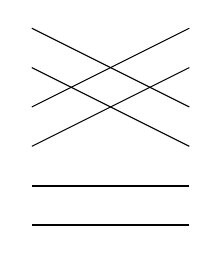
\begin{tikzpicture}[scale=0.5,>=stealth]
\draw(0,4)--(4,2);
\draw(0,5)--(4,3);
\draw(0,2)--(4,4);
\draw(0,3)--(4,5);
\draw[very thick,draw=white,double=black](0,0)--(4,0);
\draw[very thick,draw=white,double=black](0,1)--(4,1);
%\draw(2.5,-1) node {$\Sigma_1$};
\end{tikzpicture}
\caption{$\Sigma^{(2)}_1$}
\label{FigSigma2}
\end{figure}

\noindent Then if $B\in B_k$ is given by the braid word $\s_{n_1}\s_{n_2}\cdots\s_{n_m}$, we define the {\bf$p$-copy} $B^{(p)}$ of $B$ to be

$$B^{(p)} = \Sp_{n_1}\Sp_{n_2}\cdots\Sp_{n_m}$$

\noindent and we define $K^{(p)}$\todo[color=\ltblue]{eliminate this notation} to be the closure of that braid. We then have the following result.


\begin{thm}\label{main}
Let $B\in B_k$ and $B'\in B_p$, and let $B^{(p)}B'$ be the braid sum of $B^{(p)}$ and $B'$ that we get by including $B'$ into $B_{pk}$.  Suppose that there exists an augmentation $\epsilon_k\colon \A_k^{ab} \rightarrow \C$ such that $\epsilon_k\left(\Phi_B^L\right) = \operatorname{diag}{((\pm 1)^{\operatorname{w}(B)},1,\ldots,1)}$ and an augmentation $\epsilon_p\colon \A_p^{ab} \rightarrow \C$ such that $\epsilon_p\left(\Phi_{B'}^L\right) = \operatorname{diag}((\pm 1)^{w(B')},1,\ldots,1)$.  Then there exists an augmentation $\epsilon\colon \A_{pk}^{ab}\rightarrow \C$\todo[color=\ltblue]{do I want the abelianized algebra here?} such that
$$\epsilon\left(\Phi_{B^{(p)}B'}^L\right) = \operatorname{diag}((\pm 1)^{\operatorname{w}(B^{(p)}B')},1,\ldots,1)$$
\end{thm}



Among other things, this theorem implies that iterated cables of torus knots have meridional rank equal to their bridge number.  \todo[color=\ltblue]{braid rep've info needed to make well-defined} Consider a $(r,s)$-torus knot $T$ with $\gcd(r,s) = 1$ and $r<s$. $T$ has bridge number $r$ and is the closure of a braid $B$ on $r$ strands, and since all torus knots have bridge number equal to their augmentation rank (\todo[color=\ltblue]{cite cornwell}), we have that there exists an augmentation $\epsilon_T\colon \A_r\rightarrow \C$\todo[color=\ltblue]{finish this}. .  given by the braid sum of $T^{(p)}$ with a braid who's first $p$ strands form a torus knot with bridge number (and therefore augmentation rank) equal to $p$ and such that $w(T)$ is even (i.e. a $(p,q)$ torus knot, where $\gcd(p,q) = 1$, $p<q$, and $pq-q$ is even).  Theorem \ref{main} then says that this cable has augmentation rank equal to its braid index, implying that its meridional rank is equal to its bridge number.  Furthermore, we can iterate this process, taking cables of the resulting knots with augmentation rank, bridge number, and braid index all equal.\todo[color=\ltblue]{prob from Kirby list should be mentioned here}

Fix $p>0$ and let $B$ be a braid on $k$ strands. For each $1\le i\le pk$ define integers $q_i,r_i$ such that $i = q_ip + r_i$, where $0<r_i \le p$. Instrumental to the proof of Theorem \ref{main} will be the map $\psi\colon \A_{pk}^{ab} \rightarrow \A_k^{ab}\otimes \A_p^{ab}$, defined as follows (note that since \todo[color=\ltgreen]{in $\A^{ab}$ we are always making $i<j$? let's state so in background} $a_{ij}\in \A_{pk}^{ab}$, $i<j$, so we must have $q_i\le q_j$):

$$
\psi(a_{ij}) =
\left\{
     \begin{array}{lr}
       1\otimes a_{r_ir_j} & \colon q_i = q_j\\
       a_{q_i+1,q_j+1}\otimes 1 & \colon q_i<q_j,  r_i = r_j\\
       0 & \colon q_i<q_j,  r_i > r_j\\
       a_{q_i+1,q_j+1}\otimes a_{r_ir_j} & \colon q_i<q_j, r_i < r_j\\
     \end{array}
\right.
$$

\noindent Note that $\psi(a_{ij}) \in 1\otimes \A^{ab}_p$ or $\psi(a_{ij}) = 0$ if and only if $q_i = q_j$.  This homomorphism gives us a way of relating $\Phi_{B^{(p)}}^L$ to $\Phi_B^L$ via the following proposition:

\begin{prop}\label{psiofbp}
$\psi\left(\Phi_{B^{(p)}}^L\right) = \Phi_{B}^L\otimes I_p$
\end{prop} \todo[color=\ltblue]{explicit about meaning here, this is a tensor product of matrices, not of linear maps}

Note that instead of $\psi$ we could have defined a simpler homomorphism $\rho$ that would take $a_{ij}$ to $a_{q_{i+1},q_{j+1}}$ if $r_i=r_j$ and 0 otherwise, and Proposition \ref{psiofbp} would still be true. \todo[color=\ltblue]{is this obvious? "it turns out that" "follows from ideas used to prove for this psi"} The advantage of $\psi$ is that it doesn't send $a_{ij}$ to 0 if $q_i=q_j$, a fact which will be important in the proof of Theorem \ref{main}.


\begin{proof}[Proof of Theorem \ref{main}]\todo[color=\ltblue]{extend proof to w(K) odd}
Set $\epsilon = (\epsilon_k\otimes\epsilon_p)\circ\psi$.  The Chain Rule theorem gives that
\begin{equation}
(\epsilon_k\otimes\epsilon_p)\circ\psi\left(\Phi_{B^{(p)}B'}^L\right) = (\epsilon_k\otimes\epsilon_p)\psi\left(\phi_{B^{(p)}}\left(\Phi_{B'}^L\right)\right)\psi\left(\Phi_{B^{(p)}}^L\right)
\label{eqn1MainPf}
\end{equation}

Note that since the non zero or one entries of $\Phi_{B'}^L$ are products of $a_{ij}$ where $i<j \le p$, $\phi_{B^{(p)}}$ takes each of the $a_{ij}$'s in these products to $a_{i + mp, j+mp}$ for some $0\le m<k$.  We have that $\psi$ takes $a_{i + mp, j+mp}$ to $1\otimes a_{ij}$, however, so

$$\psi\left(\phi_{B^{(p)}}\left(\Phi_{B'}^L\right)\right) = \left(1\otimes \left(\Phi_{B'}^L\right)_{ij}\right)$$

\noindent By Proposition \ref{psiofbp}, we have that 

$$\psi\left(\Phi_{B^{(p)}}^L\right) = \Phi_B^L\otimes I_p$$

\noindent So returning to the right hand side of (\ref{eqn1MainPf}) we get

\begin{align*}
(\epsilon_k\otimes\epsilon_p)\psi\left(\phi_{B^{(p)}}\left(\Phi_{B'}^L\right)\right)\psi\left(\Phi_{B^{(p)}}^L\right)
    & = (\epsilon_k\otimes\epsilon_p)\left(\Phi_B^L\otimes\Phi_{B'}^L\right)\\
    & = \operatorname{diag}((-1)^{w(K)},1,\ldots,1)\otimes\operatorname{diag}((-1)^{w(K')},1,\ldots,1).
\end{align*}

\noindent But $w(K)$ is even, which also implies that $w(K^{(p)})$ is even, so the right hand side is equal to $\operatorname{diag}((-1)^{w(K^{(p)}K')},1,\ldots,1)$, as desired.

\end{proof}






%\begin{figure}[ht]
%\begin{tikzpicture}[scale=0.65,>=stealth]
%        % background
%        \foreach \c in {0,5,10} \draw (\c,1) circle (50pt);
%        \foreach \c in {0,5,10}
%                \foreach \p in {-1,1} \filldraw (\c+\p,1) circle (1.5pt);
%        \foreach \c in {0,5,10}
%                \draw   (\c+1.75,1) node {{\large $\ast$}}
%                                (\c+0.6,2.25) node {$D$}
%                                (\c-1,1) node[below] {{\small $i$}}
%                                (\c+1,1) node[below] {{\small $j$}};
%        \foreach \c in {0,10}
%                \draw   (\c,1) node {$\ldots$};
%        \filldraw       (5,1) circle (1.5pt);
%        \draw   (5,1) node[below] {{\small $k$}};
%        % on right
%        \draw[->,thick] (9,1.1) ..controls (9,1.4) and (10.7,2.2) .. (11.685,1.01);
%        \draw (10,-0.75) node[below] {{\small $\s_{i,j}\cdot c_{j,n+1}$}};
%        % on left
%        \draw[->,thick] (1,1.125) ..controls (0.75,1.625) and (-0.25,1.4) ..(-0.75,0.9)
%                                                          ..controls (-1.1,0.69) and (-1.45,0.99) ..(-1.1,1.2)
%                                                          ..controls (-0.75,1.41) and (0.7,2.2) ..(1.685,1.01);
%        \draw (0,-0.75) node[below] {{\small $\s_{i,j}\cdot c_{i,n+1}$}};
%        % in center
%        \draw[->,thick] (5,1.1) ..controls (5.2,1.3) and (5.25,1.4) ..(5.75,0.9)
%                                                        ..controls (6.1,0.69) and (6.45,0.99) ..(6.1,1.2)
%                                                        ..controls (5.2,1.75) and (4.95,1.32)   ..(5-0.75,0.9)
%                                                        ..controls (5-1.1,0.69) and (5-1.45,0.99) ..(5-1.1,1.2)
%                                                        ..controls (5-0.4,1.62) and (5.7,2.2) ..(6.685,1.01);
%        \draw (5,-0.75) node[below] {{\small $\s_{i,j}\cdot c_{k,n+1}$}};
%\end{tikzpicture}
%\caption{Computing $\Phi_{B'}^L$}
%\label{FigPhiLCalcA}
%\end{figure}


%\begin{figure}[ht]
%\begin{tikzpicture}[scale=0.65,>=stealth]
%\foreach \c in {0,10}
%	\foreach \p in {-2.5,-1.5,-.5,.5,1.5,2.5} \filldraw (\c + \p,1) circle (1.5pt);
%	
%\draw[<-,thick] (1.5,1.1) ..controls (1.5,1.9) and (-1.5,1.9) .. (-1.5,1.1);
%\draw[<-,thick] (8.5,1.1) ..controls (8.5,1.7) and (7.3,1.6) .. (7.1,1)
%										..controls (7.1,.4) and (9.3,.7) .. (10,1)
%										..controls (10.7,1.3) and (11.5,1.6) .. (11.5,1);
%\end{tikzpicture}
%\end{figure}



%\begin{prop}\label{psiofbp}
%$\psi\left(\Phi_{B^{(p)}}^L\right) = \Phi_{B}^L\otimes I_p$
%\end{prop}


\noindent We will use the following two lemmas in our proof of Proposition \ref{psiofbp}.



\begin{lem}\label{commutes}
$\psi(\phi_{\Sp_n}(a_{ij})) = (\phi_{\s_n} \otimes \id)(\psi(a_{ij}))$ for all $1\le n < k$, $1 \le i,j \le pk$.
\end{lem}

\begin{lem}\label{basecase}
$\psi\left(\Phi_{\Sp_n}^L\right) = \Phi_{\s_n}^L\otimes I_p$
\end{lem}



%Proof of psiofbp
\begin{proof} [Proof of Proposition \ref{psiofbp}]
Let $B = \s_{n_1}\cdots\s_{n_l}$, $1\le n<k$.  We will prove the proposition by inducting on $l$.  The base case is already taken care of by Lemma \ref{basecase}.  Suppose that the proposition is true for braids of length $l-1$.  Let $B' =\s_{n_1}\cdots\s_{n_{l-1}}$ Then by the Chain Rule and Lemmas \ref{commutes} and \ref{basecase}, we have that
\begin{align*}
\psi\left(\Phi_{B^{(p)}}^L\right) &= \psi\left(\phi_{B'^{(p)}}\left(\Phi_{\Sp_{n_l}}^L\right)\cdot\Phi_{B'^{(p)}}^L\right)\\
&= \left(\phi_{B'}\otimes\id\right)\left(\psi\left(\Phi_{\Sp_{n_l}}^L\right)\right)\cdot \left(\Phi_{B'}^L\otimes I_p\right)\\
&= \left(\phi_{B'}\otimes\id\right)\left(\Phi_{\s_{n_l}}^L\otimes I_p\right)\cdot \left(\Phi_{B'}^L\otimes I_p\right)\\
&= \Phi_B^L\otimes I_p
\end{align*}
\end{proof}


%FigCommutes
\todo[color=\ltblue]{make this figure smaller}
\begin{figure}[ht]
\begin{tikzpicture}[scale=0.3,>=stealth]
\foreach \y in {6}
	\foreach \p in {0,1,3,4,6,7} \filldraw (\p,\y) circle (1.5pt);
	
\foreach \a in {3.5}
	\foreach \b in {-3.5,-2.5,-.5,.5,2.5,3.5} \filldraw (\a+\b,1) circle (1.5 pt);
	
\foreach \a in {3.5,15.5,27.5,39.5}
	\foreach \b in {-3.5,-2.5,-.5,.5,2.5,3.5} \filldraw (\a+\b,-5) circle (1.5 pt);

\draw (-3.2,6) node {{\Large $\psi(\phi_{\Sp_2}($}};
\draw (8,6) node {{\Large $))$}};

\oarc{1}{6}{4}{6};
%\draw[->,thick] (1,1) ..controls (1.2,1.7) and (6.8,1.7) .. (7,1);
%\x = 12
%\draw[->,thick] (\c + 1,1) ..controls (\c + 1.2,.3) and (\c + 4.8,.3) .. (\c + 5,1);


\draw[->,thick] (1,1) ..controls (1.5,.25) and (4.5,.25) .. (5,1)
								  ..controls (5.5,1.75) and (6.5,1.75) .. (7,1);


\draw (-3.2,1) node {{$=$}};
\draw (-1.2,1) node {{\Large $\psi($}};
\draw (7.7,1) node {{\Large $)$}};

\draw (-3.2,-5) node {{$=$}};
\draw (-1.2,-5) node {{\Large $\psi($}};
\draw (44,-5) node {{\Large $)$}};

\oarc{1}{-5}{3}{-5};
\oarc{3}{-5}{4}{-5};
\oarc{4}{-5}{7}{-5};

\oarc{13}{-5}{16}{-5};
\oarc{16}{-5}{19}{-5};

\draw (9.5,-5) node {{$-$}};
\draw (21.5,-5) node {{$-$}};

\oarc{25}{-5}{27}{-5};
\oarc{27}{-5}{31}{-5};

\oarc{37}{-5}{43}{-5};

%\draw (33.5,-5) node {{$+$}};

\draw (-3.2,-11) node {{$=$}};

\foreach \x in {3.5,13.5}
	\foreach \c in {-1,0,1} \filldraw (\x + \c,-11) circle(1.5pt);
	

\draw (-1.5,-11) node {{0}};
\draw (1,-11) node {{$-$}};

\oarc{2.5}{-11}{3.5}{-11};
\oarc{3.5}{-11}{4.5}{-11};

\draw (6,-11) node {{$-$}};

\draw (8.5,-11) node {{0}};

\oarc{12.5}{-11}{14.5}{-11};

\draw (11,-11) node {{$+$}};

\draw (-3.2,-17) node {{$=$}};
\draw (-.5,-17) node {{\Large $\phi_{\s_2}($}};
\draw (3.9,-17) node {{\Large $)$}};

\foreach \x in {1.2,2.2,3.2} \filldraw (\x,-17) circle(1.5pt);

\oarc{1.2}{-17}{2.2}{-17};

\end{tikzpicture}
\caption{Computing $\psi(\phi_{\Sp_2}(a_{24}))$}
\label{FigCommutes}
\end{figure}




In the proof of Lemmas \ref{commutes} and \ref{basecase}, we will make use of some calculations of $\phi_B(a_{ij})$ for simple braids $B$.  It can easily be checked that for all $1\le m < n$, $1\le l \le n - m$, $i<j$:
\begin{equation}\label{tau}
\phi_{\tau_{m,l}}(a_{ij}) =
\left\{
     \begin{array}{lr}
       a_{i+1,j+1} & \colon m\le i<j< m+l\\
       a_{i-l,j} & \colon m<m+l=i<j\\
       a_{i,j-l} & \colon i<m<m+l=j\\
       a_{i+1,j-l} & \colon m\le i < j = m+l\\
       a_{i,j+1}-a_{i,m}a_{m,j+1} & \colon i<m\le j< m+l\\
       a_{i+1,j}-a_{i+1,m}a_{m,j} & \colon m\le i< m+l<j\\
       a_{ij} & \colon \textnormal{otherwise}
     \end{array}
\right.
\end{equation}

\noindent We also make the following definition

\noindent Let $X\subseteq \{1,\ldots,n\}$, and write the elements of a subset $Y\subseteq X$ as $y_1<\ldots <y_k$  Define
$$
 A(i,j,X) = \sum_{Y\subseteq X}(-1)^{|Y|}a_{iy_1}a_{y_1y_2}\cdots a_{y_kj}
$$
and
$$
 A'(i,j,X) = \sum_{Y\subseteq X}(-1)^{|Y|}a_{iy_k}a_{y_ky_{k-1}}\cdots a_{y_1j}
$$



\noindent and have the following lemma

%Lemma Sigma_n
\begin{lem}\label{Sigma_n}
Let $\kappa_{m,l} = \t_{m+l-1,p}\t_{m+l-2,p}\cdots\t_{m,p}$, and let $X_{m,l} = \{m-p,\ldots,m+l-p-1\}$.  Then
\todo[color=\ltblue]{check}
$$
\phi_{\kappa_{m,l}}(a_{ij}) =
\left\{
     \begin{array}{lr}
       a_{i-p,j-p} & \colon m+p\le i<j< m+l+p\\
       a_{i-p,j} &\colon m+p\le i< m+l+p\le j\\
       a_{i,j-p} & \colon i<m<m+p\le j<m+l+p\\
       a_{i+l,j+l} &\colon m\le i<j<m+p\\
       A'(i+l,j-p,X_{m,l}\setminus (j-p)) & \colon m\le i<m+p\le j <m+l+p\\
       A(i,j+l,X_{m,l}) & \colon i<m\le j <m+p<m+l+p\\
       A'(i+l,j,X_{m,l}) & \colon m\le i <m+p<m+l+p\le j\\
       a_{ij} & \colon \textnormal{otherwise}
     \end{array}
\right.
$$
\end{lem}

\noindent Note that letting $l=p$ and $m=p(n-1) + 1$ gives us $\phi_{\Sigma_n}(a_{ij})$ as a special case of this lemma.



%proof of commutes
\begin{proof} [Proof of Lemma \ref{commutes}]
The first four cases as well as the last case from Lemma \ref{Sigma_n} can be checked easily.  Consider the sixth case.  Let $\a_i  = np-p+r_i$, and we have that
\begin{align*}
&\psi\left(\phi_{\Sp_n}(a_{ij})\right) \\
&= \psi\left(A(i,j+p,\{np-p+1,\ldots,np\})\right)\\
&= \sum_{Y\subseteq \{np-p+1,\ldots,np\}}(-1)^{|Y|}\psi\left(a_{iy_1}a_{y_1y_2}\cdots a_{y_k,j+p}\right)\\
&= \sum_{Y\subseteq \{\a_i,\ldots,\a_j\}}(-1)^{|Y|}\psi\left(a_{iy_1}a_{y_1y_2}\cdots a_{y_k,j+p}\right)\\
&= \psi\left(a_{i,j+p} - a_{i,\a_i}a_{\a_i,j+p}\right)\\
& \;\;\;\;+ \sum_{y=\a_i+1}^{\a_j}\sum_{Y\subseteq \{y+1,\ldots,\a_j\}}(-1)^{|Y|+1}\psi\left(a_{iy}a_{yy_1}\cdots a_{y_k,j+p}\right) + (-1)^{|Y|}\psi\left(a_{i,\a_i}a_{\a_i,y}a_{yy_1}\cdots a_{y_k,j+p}\right)\\
&= \psi\left(a_{i,j+p} - a_{i\a_i}a_{\a_i,j+p}\right)\\
& \;\;\;\;+ \sum_{y=\a_i+1}^{\a_j}\sum_{Y\subseteq \{y+1,\ldots,\a_j\}}(-1)^{|Y|}\psi\left(a_{i,\a_i}a_{\a_i,y} - a_{iy}\right)\psi\left(a_{yy_1}\cdots a_{y_k,j+p}\right)\\
&= \psi\left(a_{i,j+p} - a_{i\a_i}a_{\a_i,j+p}\right)\\
\end{align*}

\todo[color=\ltblue,inline]{change $\a_i,\ldots,\a_j$ to $\a_i,\a_i+1,\ldots,\a_j$ and mention why the transition to these things happens on that line}


\todo[color=\ltblue,inline]{show why term in second-to-last RHS is zero}
\todo[color=\ltblue]{note $\psi$ is defined this way basically so that this is zero}

\noindent Note that, since we're in the sixth case, $q_j + 1 = n$.  If $r_i = r_j$, then 
$$\psi\left(a_{i,j+p} - a_{i\a_i}a_{\a_i,j+p}\right) = \left(a_{q_i+1,n+1} - a_{q_i+1,n}a_{n,n+1}\right)\otimes 1 = (\phi_{\s_n} \otimes \id)(\psi(a_{ij}))$$
If $r_i < r_j$, then
\begin{align*}
\psi\left(a_{i,j+p} - a_{i\a_i}a_{\a_i,j+p}\right) &= \left(a_{q_i+1,n+1}\otimes a_{r_ir_j} - a_{q_i+1,n}a_{n,n+1}\otimes a_{r_ir_j}\right)\\
&= \left(a_{q_i+1,n+1} - a_{q_i+1,n}a_{n,n+1}\right)\otimes a_{r_ir_j}\\
&= (\phi_{\s_n} \otimes \id)(\psi(a_{ij}))
\end{align*}
Finally, if $r_i > r_j$, then
$$\psi\left(a_{i,j+p} - a_{i\a_i}a_{\a_i,j+p}\right) = 0 = (\phi_{\s_n} \otimes \id)(\psi(a_{ij}))$$

The proof for the seventh case goes exactly as the proof for the sixth case except with all $i$'s replaced with $i+p$, all $(j+p)$'s replaced with $j$, all $y_i$'s replaced with $y_{k+1-i}$, and with $\a_i$ and $\a_j$ swapped.  The proof for the fifth case goes exactly as the proof for the seventh, except that $j-p$ is removed from the set that $Y$ is a subset of in all the sums.


%This gives that
%
%$$\psi\left(\phi_{\Sp_n}(a_{ij})\right) = \psi\left(a_{i+p,j} - a_{i+p,\a_j}a_{\a_j,j}\right)$$
%
%Since we're in the fifth case, $q_i + 1 = n$.  If $r_i = r_j$, then
%
%$$\psi\left(a_{i+p,j} - a_{i+p,\a_j}a_{\a_j,j}\right) = \left(a_{n+1,q_j+1} - a_{n+1,n}a_{n,q_j+1}\right)\otimes 1 = (\phi_{\Sp_n} \otimes \id)(\psi(a_{ij}))$$

\end{proof}



%proof of basecase
\begin{proof} [Proof of Lemma \ref{basecase}]
We can extend the definition of $\psi$ to be from the free module over $\A_{pk}$ generated by $\{a_{i*}|1\le i\le pk\}$ to the free module over $\A_{k}\otimes \A_{p}$ generated by $\{a_{i*}|1\le i\le k\}$ by defining $\psi(a_{i*}) = a_{i*}$ and extending by linearity.  Then the statement of the lemma is equivalent to saying that for all $1\le i\le pk$, the coefficient of $a_{j*}$ in $\psi\left(\phi_{\Sp_n}(a_{i*})\right)$ is equal to 0 unless $r_j = r_i$, in which case it is equal to the coefficient of $a_{q_j*}$ in $\phi_{\s_n}(a_{q_i*})$.  If $q_i + 1 \ne n$, this fact can be easily checked.  In the case that $q_i + 1 = n$, we have that
$$\psi\left(\phi_{\Sp_n}(a_{i*})\right) = \psi\left(A(i+p,*,\{np-p+1,\ldots,np\}\right)$$
\noindent which is equal to
$$\psi(a_{i+p,*} - a_{i+p,\a_i}a_{\a_i,*}) = a_{i+p,*} - a_{q_i,q_i+1}a_{\a_i,*}$$
by the same argument that was used in Lemma \ref{commutes}.  The coefficients of the $a_{j*}$ are equal to the coefficients of the $a_{q_j*}$ in $\phi_{\s_n}(a_{q_i*})$, so we're done.
\end{proof}














%$$%out of date
%\phi_{\tau_{m,l}}(a_{ij}) =
%\left\{
%     \begin{array}{lr}
%       a_{i-1,j-1} & \colon m<i<j\le m+l\\
%       a_{i,j-1} & \colon i<m<j\le m+l\\
%       a_{i-1,j} & \colon m<i\le m+l<j\\
%       A'(i+l,j-1,X\setminus \{j-1\}) & \colon m=i<j\le m+l\\
%       A'(i+l,j,X) & \colon m=i<m+l<j\\
%       A(i,j+l,X) & \colon i<j=m < m+l\\
%       a_{ij} & \colon \textnormal{otherwise}
%     \end{array}
%\right.
%$$


%\begin{proof}
%\begin{proof} %out of date
%The first three cases as well as the last can be checked easily.  We prove the remaining cases by inducting on $l$.
%
%
%Consider the fourth case, $m=i<j\le m+l$.  For the base case, we have $l=1$, $\t_{m,l} = \s_m$, and $j=m+1$.  We have
%$$\phi_{\s_m}(a_{ij}) = \phi_{\s_m}(a_{m,m+1})  = a_{m+1,1} = A'(i+1,j-1,\{\})$$
%
%For $l>1$, we have
%\begin{align*}
%\phi_{\t_{m,l}}(a_{ij}) &= \phi_{\s_{m+l-1}}(\phi_{\t_{m,l-1}}(a_{mj}))\\
%&= \phi_{\s_{m+l-1}}\left(A'(i+l-1,j-1,X\setminus\{j-1\})\right)\\
%&= \sum_{Y\subseteq \{m,\ldots,m+l-2\}\setminus \{j-1\}} (-1)^{|Y|}\phi_{\s_{m+l-1}}\left(a_{m+l-1,y_k}a_{y_ky_{k-1}}\cdots a_{y_1,j-1}\right)\\
%&= \sum_{Y\subseteq \{m,\ldots,m+l-2\}\setminus \{j-1\}} (-1)^{|Y|}\left(a_{m+l,y_k} - a_{m+l,m+l-1}a_{m+l-1,y_k}\right)a_{y_ky_{k-1}}\cdots a_{y_1,j-1}\\ 
%&= \sum_{Y\subseteq \{m,\ldots,m+l-1\}\setminus \{j-1\}} (-1)^{|Y|}a_{m+l,y_k}a_{y_ky_{k-1}}\cdots a_{y_1,j-1}\\ 
%&= A'(i+l,j-1,X\setminus \{j-1\})
%\end{align*}






%Consider the fifth case, $m=i<m+l<j$.  For the base case, we have $l=1$, and $\tau_{m,l} = \s_m$.  We have
%$$\phi_{\s_m}(a_{ij}) = \phi_{\s_m}(a_{mj})  = a_{m+1,j} - a_{m+1,m}a_{mj} = A'(m+1,j,\{m\})$$
%
%For $l>1$, we have
%\begin{align*}
%\phi_{\tau_{m,l}}(a_{mj}) &= \phi_{\s_{m+l-1}}(\phi_{\tau_{m,l-1}}(a_{mj}))\\
%&= \phi_{\s_{m+l-1}}\left(\sum_{Y\subseteq \{m,\ldots,m+l-2\}}(-1)^{|Y|}a_{m+l-1,y_k}a_{y_ky_{k-1}}\cdots a_{y_1,j}\right)\\
%&= \sum_{Y\subseteq \{m,\ldots,m+l-2\}} (-1)^{|Y|}\phi_{\s_{m+l-1}}\left(a_{m+l-1,y_k}a_{y_ky_{k-1}}\cdots a_{y_1j}\right)\\
%&= \sum_{Y\subseteq \{m,\ldots,m+l-2\}} (-1)^{|Y|}\left(a_{m+l,y_k} - a_{m+l,m+l-1}a_{m+l-1,y_k}\right)a_{y_ky_{k-1}}\cdots a_{y_1j}\\ 
%&= \sum_{Y\subseteq \{m,\ldots,m+l-1\}} (-1)^{|Y|}a_{m+l,y_k}a_{y_ky_{k-1}}\cdots a_{y_1,j}\\ 
%&= A'(i+l,j,\{m,\ldots,m+l-1\})
%\end{align*}
%
%
%
%
%Consider the sixth case, $i<j=m<m+l$. For the base case, we have $l=1$, and $\tau_{m,l} = \s_m$.  We have 
%$$\phi_{\s_m}(a_{im}) = a_{i,m+1} - a_{im}a_{m,m+1} = A(i,m+1,\{m\})$$
%For $l>1$, we have
%\begin{align*}
%\phi_{\tau_{m,l}}(a_{im}) &= \phi_{\s_{m+l-1}}(\phi_{\tau_{m,l-1}}(a_{im}))\\
%&= \phi_{\s_{m+l-1}}\left(\sum_{Y\subseteq \{m,\ldots,m+l-2\}}(-1)^{|Y|}a_{i,y_1}a_{y_1y_2}\cdots a_{y_k,m+l-1}\right)\\
%&= \sum_{Y\subseteq \{m,\ldots,m+l-2\}} (-1)^{|Y|}\phi_{\s_{m+l-1}}\left(a_{iy_1}a_{y_1y_2}\cdots a_{y_k,m+l-1}\right)\\
%&= \sum_{Y\subseteq \{m,\ldots,m+l-2\}} (-1)^{|Y|}a_{iy_1}a_{y_1y_2}\cdots a_{y_{k-1}y_k} \left(a_{y_k,m+l} - a_{y_k,m+l-1}a_{m+l-1,m+l}\right)\\ 
%&= \sum_{Y\subseteq \{m,\ldots,m+l-1\}} (-1)^{|Y|}a_{iy_1}a_{y_1y_2}\cdots a_{y_k,m+l}\\ 
%&= A(i,j+l,X)
%\end{align*}



%The proofs of fifth and sixth cases are each similar and slightly simpler.  In each case we apply induction and manipulate summations as above.
%\end{proof}
%\end{proof}






\begin{proof} [Proof of Lemma \ref{Sigma_n}]\todo[color=\ltblue,inline]{add other cases}
The first four cases as well as the eighth can be easily checked.  We will prove the remaining cases by induction on $l$.  Consider the sixth case.  The base case is covered by (\ref{tau}).  For the inductive step, we have that

\begin{align*}
\phi_{\k_{m,l}}(a_{ij}) &= \phi_{\t_{m,p}}\left(\phi_{\k_{m+1,l-1}}(a_{ij})\right)\\
&= \phi_{\t_{m,p}}\left(A(i-l+1,j,X_{m+1,l-1})\right)\\
&= \sum_{Y\subseteq \{m+p+1,\ldots,m+l+p-1\}} (-1)^{|Y|} \phi_{\t_{m,p}}\left(a_{i-l+1,y_1}a_{y_1y_2}\cdots a_{y_k,j}\right)\\
&= \sum_{Y\subseteq \{m+p+1,\ldots,m+l+p-1\}} (-1)^{|Y|} \left(a_{i-l,y_1}-a_{i-l,m+p}a_{m+p,y_1}\right)a_{y_1y_2}\cdots a_{y_k,j}\\
&= \sum_{Y\subseteq \{m+p,\ldots,m+l+p-1\}} (-1)^{|Y|} a_{i-l,y_1}a_{y_1y_2}\cdots a_{y_k,j}\\
&= A(i-l,j,X_{m,l})
\end{align*}



\end{proof}







%\begin{thm}\label{main}\todoit make numbering match
%Suppose that there exists an augmentation $\epsilon_k\colon \A_k \rightarrow \C$ such that $\epsilon_k\left(\Phi_B^L\right) = \operatorname{diag}{((\pm 1)^{\operatorname{w}(K)},1,\ldots,1)}$ and an augmentation $\epsilon_p\colon \A_p \rightarrow \C$ such that $\epsilon_p\left(\Phi_{B'}^L\right) = \operatorname{diag}((\pm 1)^{w(K')},1,\ldots,1)$, and furthermore that $w(K)$ is even.  Then there exists an augmentation $\epsilon\colon \A_{pk}\rightarrow \C$ such that
%$$\epsilon\left(\Phi_{B^{(p)}B'}^L\right) = \operatorname{diag}((\pm 1)^{\operatorname{w}(K^{(p)}K')},1,\ldots,1)$$
%\end{thm}




\bibliography{AugsCables_refs}
\bibliographystyle{alpha}
\end{document}
